\subsubsection{Les tâches de test des capacités du sujets}

\paragraph{Le gaborium}Cette tâche utilise également des \glspl{gabor} comme stimulus. Un écran rempli d'une multitude de gabors de tailles et d'orientations différentes est montré
au sujet. Tous les distracteurs sont des gabors avec une direction et une vitesse de mouvement constante. La cible est un gabor dont la direction et la vitesse changent constamment.
Dans cette tâche, le sujet doit cliquer sur la cible avec la souris des qu'il l'aperçoit. La cible disparaît alors et une autre cible fait son apparition après un laps de temps
variable. L'œil droit du sujet est traqué à l'aide d'un eye tracker Eyelink. Il doit également appuyer sur la barre espace s'il sent qu'il n'est plus concentré sur la tâche de Gaborium.

\begin{figure}[H]
    \begin{center}
    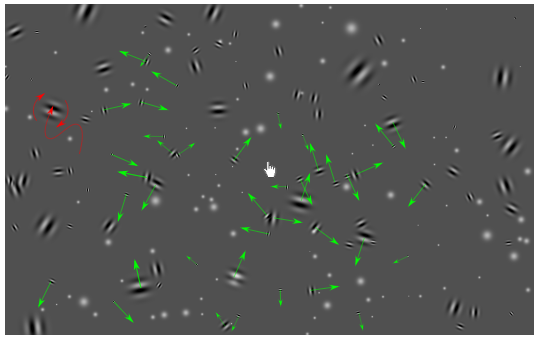
\includegraphics[width=11cm]{gaborium.png}
    \end{center}
    \caption{Gaborium avec les directions de certains gabors affichées}
\label{Gaborium}
\end{figure}

\paragraph{Traitement des données}Les données à observer pour l'analyse de l'attention sur la tâche sont les temps de réaction et la fréquence à laquelle le sujet appuie sur la barre
espace. La tâche ayant été créée récemment, elle n'est pas encore parfaite : peu de gens voire personne n'appuie sur la barre espace. Nous n'avons donc pas de données exploitables.
On a donc essayé d'enregistrer le mouvement des yeux ainsi que le diamètre pupillaire. Nous savons qu'il existe un lien entre ce diamètre et l'aspect émotionnel et attentionnel d'une
personne : plus le diamètre est grand et plus la personne est attentive. Néanmoins, on sait aussi que le diamètre pupillaire change aussi selon la luminosité. Dans les données, nous
avons donc des fluctuations rapides représentant le changement de luminosité entre le fond gris et les gabors noirs, et des fluctuations plus lentes représentant le niveau attentionnel
du sujet.


\paragraph{Les multiplications}Dans cette tâche, le joueur voit apparaître la multiplication d'un nombre à deux chiffres par un autre chiffre pendant quelques secondes. Ensuite, la
multiplication disparaît, remplacée par 4 propositions de réponses plus ou moins proches qui n'apparaissent également que durant quelques secondes. Il doit alors choisir la bonne
réponse à l'aide du pavé numérique. Le sujet doit trouver des solutions pour calculer rapidement le résultat et ne pas se faire submerger. Il peut par exemple essayer de trouver le
chiffre des unités de la réponse et en déduire la bonne proposition.

\paragraph{Traitement des données}On analyse les bonnes réponses du sujet mais également ses temps de réponse. Lorsqu'il a faux, on peut analyser quelle réponse il a choisi : si le
chiffre des unités est le bon, c'est qu'il a probablement commencé à faire le calcul mais n'a pas pu le faire complètement. Sinon c'est qu'il est possible qu'il ait répondu au hasard.


\paragraph{Rôle de ces tâches}Le gaborium est censé représenter une tâche facile dans la figure \ref{DifficultyAndAttention}. C'est une tâche qui n'est pas assez difficile pour le
sujet et qui, si notre théorie est bonne, doit le faire vagabonder. La tâche des multiplications représente à l'inverse une tâche si difficile qu'elle doit faire décrocher le sujet.
Ces deux tâches pourraient permettre d'évaluer les capacités du sujet pour savoir comment adapter la difficulté des tâches d'entrainement pour que celui-ci soit optimal.